\chapter{Results and discussion}\label{cha:results}
In this chapter the results of the experiments detailed in the previous chapter are shown and discussed. The first section deals with pruning-related results. The next section is about categorical attributes and the final section pertains to the binary tree issue.

\section{Pruning}
In \autoref{cha:software_new}, pruning extensions were added to scikit-learn's decision tree implementations. More specifically, Reduced Error Pruning (REP) and Error Based Pruning (EBP) were implemented. In this section we evaluate how these pruning extensions affect the size of the tree (i.e., the number of nodes), the performance in terms of accuracy and the fitting and prediction speed.

%TODO next, Weka
\subsection{Tree size}
The mean size of the trees is shown as a heatmap in \autoref{fig:heat_nodes} for each dataset and each scikit-learn configuration. The values have been normalized by the mean size per dataset of unpruned trees. As such, the \emph{none} row which indicates that no pruning was performed is filled with 100\% values.

\begin{figure}[htp]
    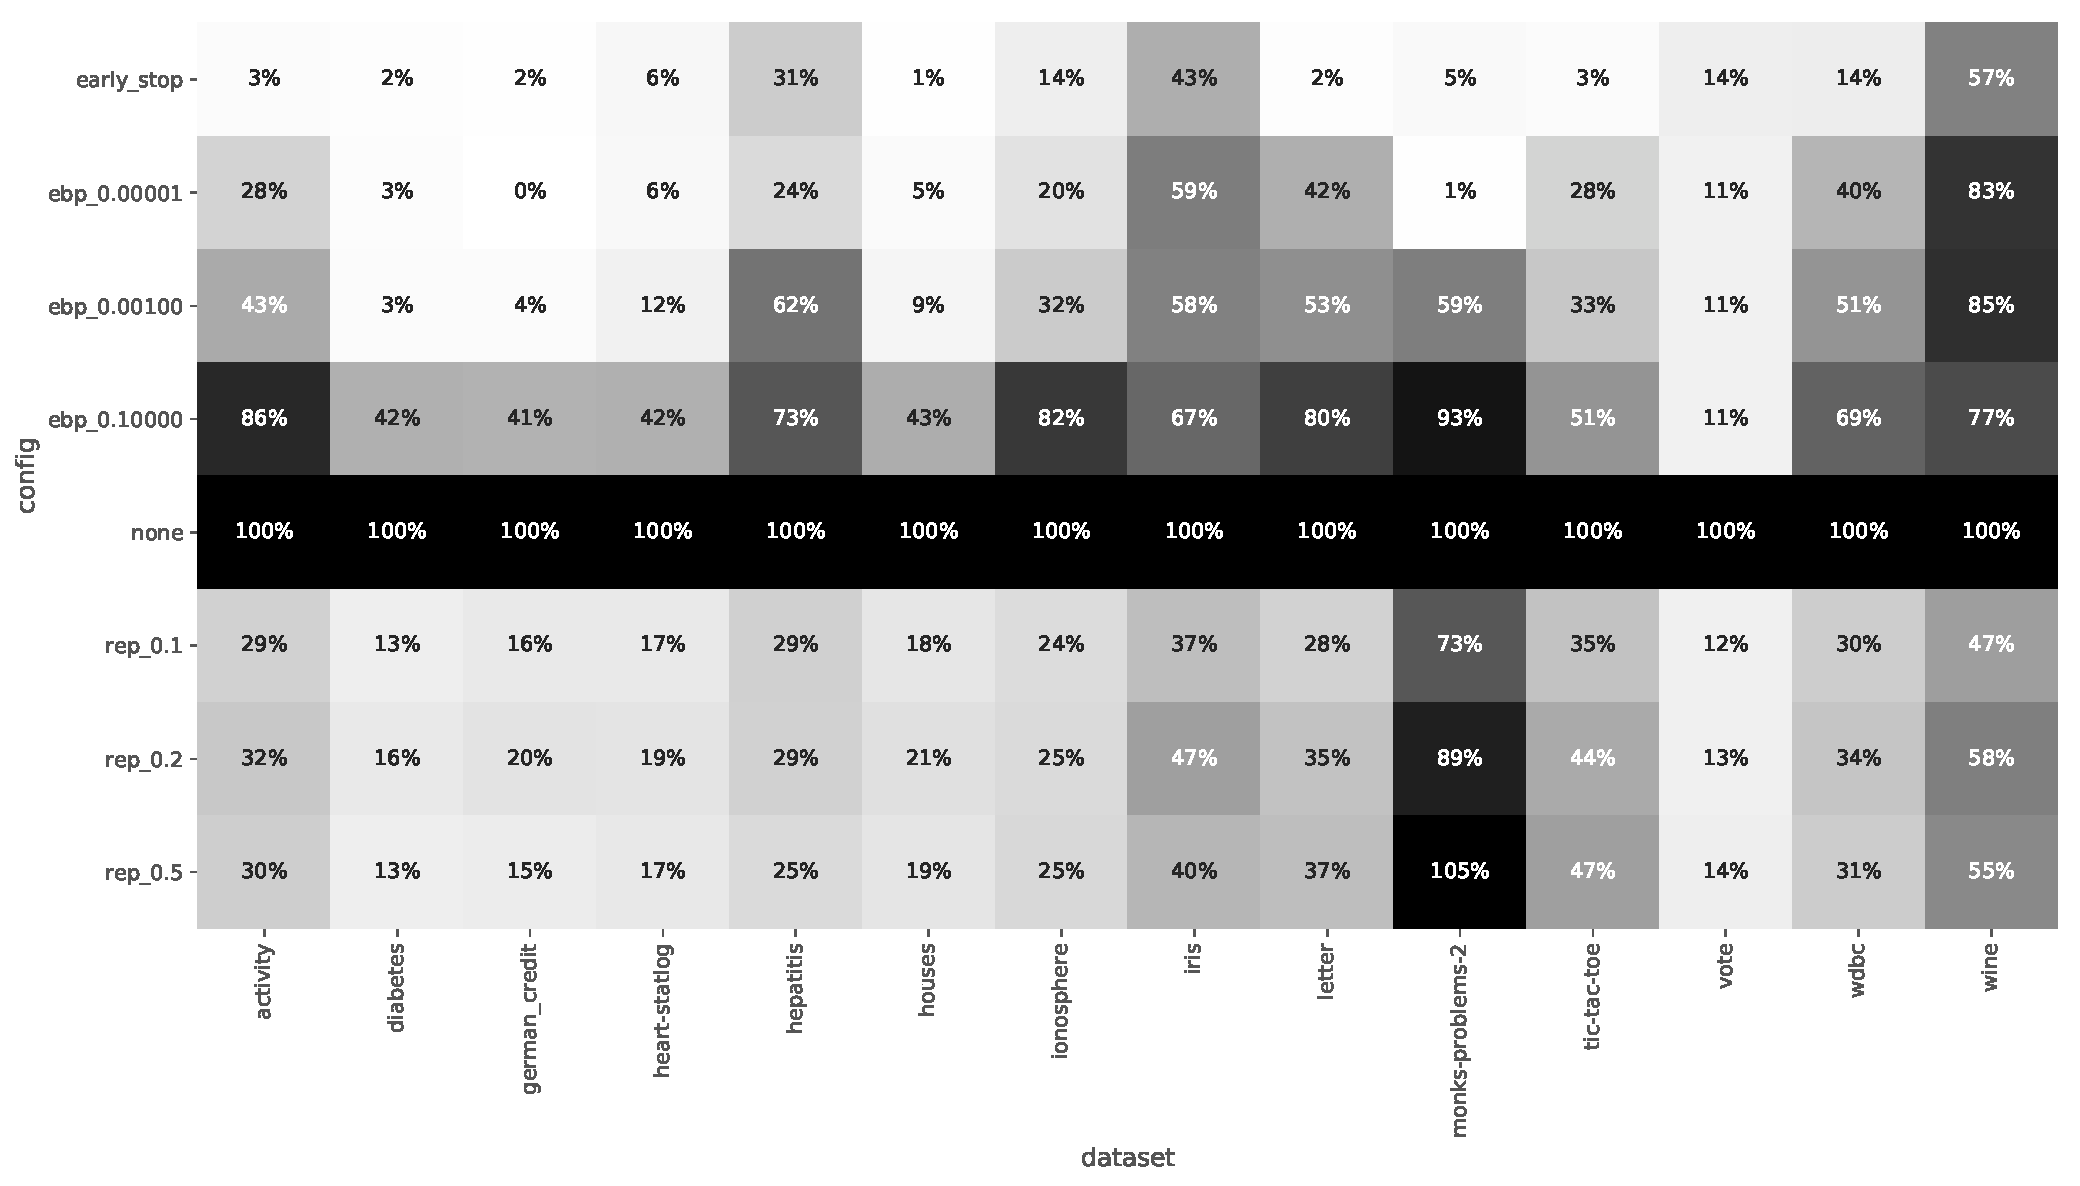
\includegraphics[width=\textwidth]{img/heatmap_n_nodes.pdf}
    \caption{Mean tree size per scikit-learn configuration and per dataset. The values have been normalized by the mean size per dataset of unpruned trees. Weka results are not included in this heatmap. The colour scale goes from 0\% (white) to 100\% (black).}%
    \label{fig:heat_nodes}
\end{figure}

One value exceeds 100\%. This is possible because the pruned trees are not derivatives of the unpruned trees. They are simply two different configurations that are tested independently of each other. In this specific case, Reduced Error Pruning was used with a validation set size of 50\%. Since 10\% of the total was already set apart in the cross-validation procedure, only 45\% of the original data was left to train the tree. This can profoundly change the tree structure, including its size before pruning. This size is unknown, but it must have been larger than the tree size of an unpruned tree trained on 90\% of the original data. Even after pruning, the former tree turned out to be larger than the latter.

The next observation is that the other rows in the heatmap are quite light, meaning that in general the tree sizes have been reduced greatly by the various pruning strategies. For Error Based Pruning, the confidence factor plays a large role in the amount of pruning that is performed. A very low confidence factor of $10^{-5}$ results in very aggressive pruning while a factor of $10^{-1}$ results in very little pruning. The validation set size of Reduced Error Pruning on the other hand does not have a clear impact on pruning aggression. A larger validation set simply implies that the error estimates become more reliable, but not that they move in any particular direction.

Specifically for scikit-learn, a pseudo-pruning configuration is added that uses an early stopping criterion based on the \texttt{min\_samples\_leaf} parameter instead. This is what scikit-learn users do when pruning algorithms are unavailable. As discussed earlier, it is not easy to find a good value for this hyperparameter that performs similarly across a variety of datasets. In this case the result is very aggressive pruning except for datasets wine, iris and hepatitis. This is simply because the unpruned trees of these datasets were small to begin with, and this criterion aims for a low absolute number of nodes. The other configurations also score worse on these datasets because there is less potential for pruning if there are fewer nodes to start with.

% activity             580.94
% diabetes             233.28
% german_credit        329.32
% heart-statlog         78.22
% hepatitis             15.40
% houses               499.02
% ionosphere            37.06
% iris                  16.28
% letter              3916.08
% monks-problems-2      91.76
% tic-tac-toe          143.10
% vote                  26.32
% wdbc                  34.78
% wine                  15.00

The previous heatmap only showed results obtained from the scikit-learn configurations. The next step is to compare these results with those of Weka. \autoref{fig:heat_nodes_diff} visualizes the differences in number of nodes.

\begin{figure}[htp]
    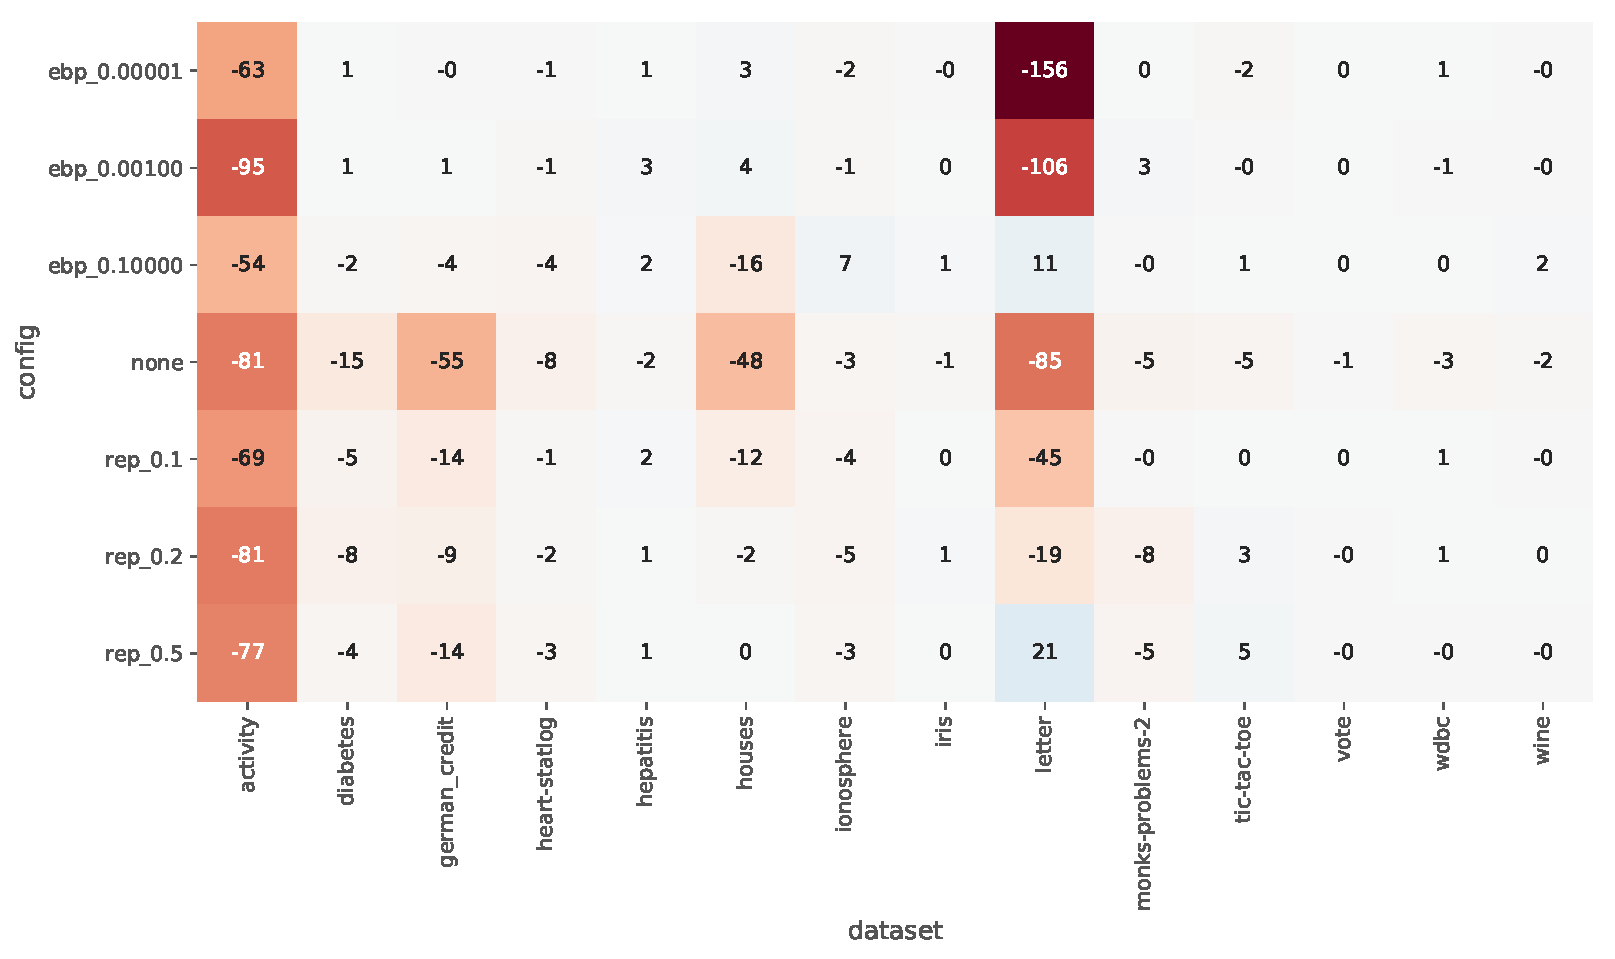
\includegraphics[width=\textwidth]{img/heatmap_n_nodes_diff.pdf}
    \caption{Absolute values of the differences between scikit-learn and Weka mean tree size per configuration and per dataset.}%
    \label{fig:heat_nodes_diff}
\end{figure}

Most of the differences are minimal. The only configuration with some larger differences is the one where pruning is not applied. The previous heatmap showed us that mean unpruned tree size can be a multiple of any mean pruned tree size. Consequently, the differences in size between unpruned trees are also larger in absolute numbers. Also note that this configuration does not contain custom code developed for this thesis. Additionally, it is proof that CART and C4.5 (and their respective implementations) do not produce the exact same trees, even when configured very similarly.

Column-wise, the letter, activity datasets --- and to a lesser extent also houses and german\_credit datasets --- stand out. These are the datasets which on average generate the largest unpruned trees, yet percentage-wise the effect of pruning on them is average. As a result, their pruned trees are on average also large. This explains the larger absolute differences. When expressed relatively in percentages, the heatmap does not show any remarkable discrepancy between these four datasets and the rest.

\subsection{Accuracy}
\autoref{fig:heat_acc} shows a heatmap of the mean accuracy per scikit-learn configuration and per dataset. The most important observation here is that all configurations except for early stopping behave very similarly, despite large differences in the amount of pruning. Of course this is the purpose of pruning: reduce model complexity without affecting performance too much. This goal is clearly accomplished. At the same time, a strong contrast with the performance of the early stopping criterion is revealed. Across the board, it performs worse than all real pruning configurations.

\begin{figure}[htp]
    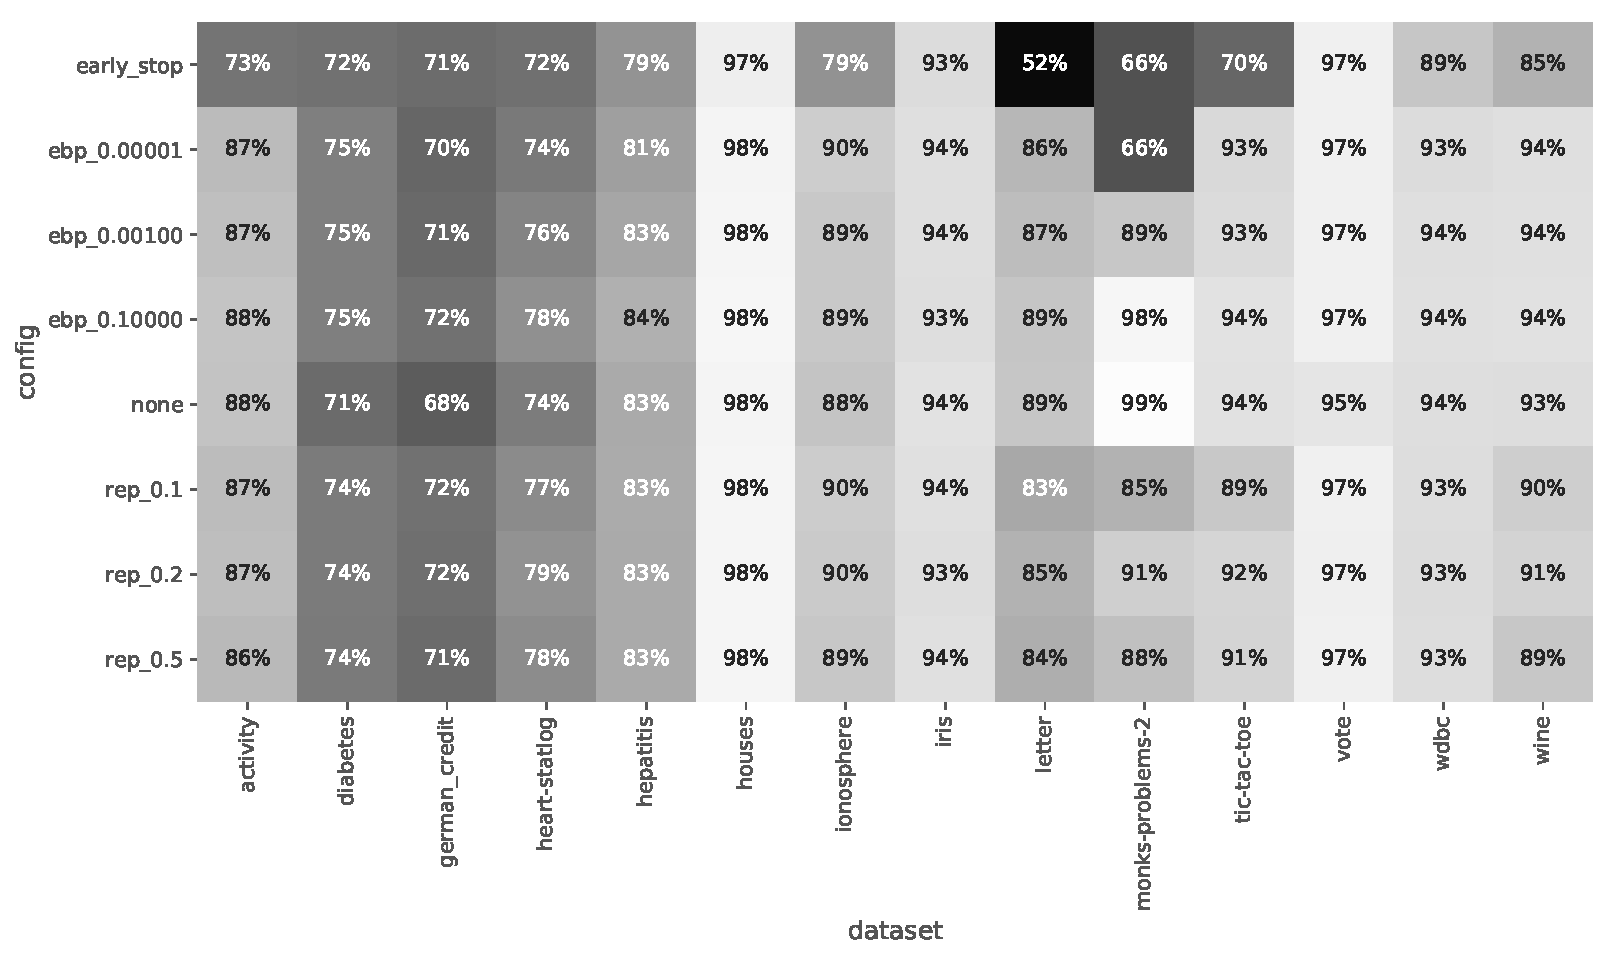
\includegraphics[width=\textwidth]{img/heatmap_accuracy.pdf}
    \caption{Mean accuracy per scikit-learn configuration and per dataset. Weka results are not included in this heatmap. The colour scale goes from 50\% (black) to 100\% (white).}%
    \label{fig:heat_acc}
\end{figure}

This heatmap also clearly shows that accuracy is strongly dependent on the dataset. Not all datasets can be modelled equally well with trees. Differences in class balance also exist between datasets. Accuracy as a metric can be biased when the classes are strongly unbalanced. Alternative metrics such as the F1-score are better suited in such scenarios. A similar heatmap as shown here was generated using this F1-score, but it is not included because the results were almost identical.

%Activity dataset problem could not be reproduced -> very good accuracy even without pruning

\section{Categorical attributes}

\section{Binary versus non-binary trees}
% Weka: binary vs non binary - significant differences
%   binary -> non-binary
%   tic-tac-toe: 
%       41.36 -> 10 nodes
%       21.18 -> 7 leaves
%       92.79 -> 68.96 accuracy
%       0.93 -> 0.71 F1
%   monks: always tree with only root node, no F1 score
%   activity: 85.66 -> 84.43 accuracy (no significant difference in F1)
% ==> non-binary same or disadvantage

\section{Conclusion}
